\documentclass[12pt, letterpaper]{report}
\usepackage{amsmath,amsthm,amssymb}
\usepackage{mathtext}
\usepackage{graphicx}
\graphicspath{{pictures/}}
\DeclareGraphicsExtensions{.jpg}
\usepackage[T1,T2A]{fontenc}
\usepackage{lmodern}
\usepackage[utf8]{inputenc}
\usepackage[english,russian]{babel}
\usepackage[usenames,dvipsnames]{color}
\usepackage{alltt}
\usepackage{microtype}

\makeatletter
\newcommand{\anonchapter}[1]{\chapter*{#1}\addcontentsline{toc}{chapter}{#1}}
\renewcommand\@biblabel[1]{#1.\hfil}
\makeatother

\begin{document}
	
	\begin{titlepage}
		
		\begin{center}
			Министерство науки и высшего образования Российской Федерации
		\end{center}
		
		\begin{center}
			Федеральное государственное автономное образовательное учреждение высшего образования \\
			Национальный исследовательский Нижегородский государственный университет им. Н.И. Лобачевского
		\end{center}
		
		\begin{center}
			Институт информационных технологий, математики и механики
		\end{center}
		
		\vspace{4em}
		
		\begin{center}
			\textbf{\LargeОтчет по лабораторной работе} \\
		\end{center}
		\begin{center}
			\textbf{\Large«Сортировка Шелла с простым слиянием»} \\
		\end{center}
		
		\vspace{4em}
		
		\newbox{\lbox}
		\savebox{\lbox}{\hbox{text}}
		\newlength{\maxl}
		\setlength{\maxl}{\wd\lbox}
		\hfill\parbox{7cm}{
			\hspace*{5cm}\hspace*{-5cm}\textbf{Выполнила:} \\ студентка группы 381808-1 \\ Бурмистрова Е. О.\\
			\\
			\hspace*{5cm}\hspace*{-5cm}\textbf{Проверил:}\\ доцент кафедры МОСТ, \\ кандидат технических наук \\ Сысоев А. В.\\}
		\vspace{\fill}
		
		\begin{center} Нижний Новгород \\ 2020 \end{center}
		
	\end{titlepage}
	
	\setcounter{page}{2}
	
	% Содержание
	\tableofcontents
	\newpage
	

\anonchapter{Введение}
На данный момент существует множество различных алгоритмов сортировки.
Подобное разнообразие объясняется вариативностью задач и условий их выполнения.
Сортировки, имеющие сложность \(N^2\)
 хорошо справляются с небольшими наборами
данных (и, к тому же, обычно не требуют использования дополнительной памяти), а
сортировки со сложностью исполнения \(N(\log N)\) подойдут для больших объемов.

Сортировка Шелла - одна из самых простых в понимании и реализации среди быстрых
сортировок. Эта сортировка используется в ядре Linux, и в, как минимум, в одной библиотеке
С её код используется для стандартной функции qsort().

Обычно сортировка Шелла часто даже быстрее теоретически более быстрых по порядку
методов и начинает чуть уступать им лишь, при обработке довольно больших массивов
(порядка 10-в миллионов элементов). Этой сортировке совершенно не нужна дополнительная
память и она стабильно ведёт себя для самых разных вариантов заполнения данных, выгодно
отличаясь этим от быстрых сортировок.

\chapter*{Постановка задачи}
В данной лабораторной работе было необходимо
\begin{itemize}
\item реализовать параллельный метод сортировки Шелла на языке С++ с
использованием библиотеки MPI.
\item реализовать последовательный алгоритм сортировки Шелла
\item сравнить эффективность алгоритмов
\end{itemize}

\chapter*{Метод решения}
Сортировка Шелла представляет собой усовершенствованный алгоритм сортировки
вставками. Идея метода Шелла состоит в сравнениях и перестановках элементов,
расположенных не только рядом, но и на определённом расстоянии друг от друга в
сортируемом массиве. Процесс сортировки включает несколько этапов, на каждом из
которых производится последовательная сортировка вставками нескольких подсписков
элементов, выделяемых в исходном массиве. Например, если в подсписок входит
каждый k-й элемент, то получаем k таких подсписков (величина k называется шагом
сортировки). Этим достигается частичная упорядоченность элементов массива, что
повышает эффективность алгоритма сортировки вставками. Затем величина k
уменьшается и процедура повторяется. Окончательный результат получают при k=1.
Также необходимо учитывать,что количество подмассивов может быть больше
используемого количества процессов. Для того, чтобы в данной ситуации обработать
все объекты, необходимо обернуть циклы прохода по массиву циклом,
контролирующим число выделяемых процессов.
Для получения отсортированных данных (за исключением 0 процесса, т.к.,его
элементы не отправляются в другой процесс для сортировки) реализуется отдельный
цикл, в котором полученные из процессов данные размещаются в исходном векторе в
искомом порядке.

\chapter*{Схема распараллеливания}
На начальном этапе имеем некоторый массив (созданный вручную или
сгенерированный), который хранится в 0 процессе.

Если общее количество процессов больше 1 и размер исходного массива больше 1,
начинаем процесс параллельной сортировки Шелла, а именно:
\begin{enumerate} 
\item Выбираем начальный шаг (в данном случае он кратен 2ум)
\item Заводим внешний цикл while, который будет работать до тех пор, пока шаг
нашей сортировки не станет = 0.
\item Внутри цикла while заведём цикл do{}while для корректного разбиения
проходов по процессам.
\item Теперь с текущим шагом проходим по массиву несколько раз и каждый из
наборов отправляем в отдельный процесс
\item В каждом из процессов сортируем данные и отправляем их обратно в 0 процесс
для размещения элементов.

\end{enumerate}
На конкретном примере это выглядит так:
\par
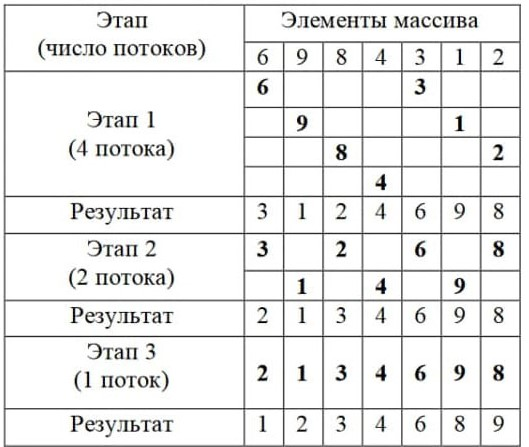
\includegraphics[scale=0.7]{shell}
\chapter*{Описание программной реализации}
В данной работе реализованы 4 метода :
\begin{alltt}
std::vector<int> gen_input(int sz) {} - для генерации вектора заданной 
длины,состоящего из рандомных значений.

std::vector<int> Sequential_Shell(std::vector<int> vec) {} - для
последовательного исполнения алгоритма Шелла над вектором данных 
заданной длины.

std::vector<int> Sequential_sort(std::vector<int> vect) {} - для последовательного выполнения сортировки Вставками над вектором данных заданной длины.

std::vector<int> Parallel_sort(std::vector<int> vect) {} - для параллельного исполнения метода Шелла над вектором заданной длины.
\end{alltt}
\chapter*{Подтверждение корректности}
Для подтверждения корректности работы были созданы 5 тестов.
\begin{alltt}
TEST(Parallel_sort, sort_random_vect) {}
TEST(Parallel_sort, compare_time_sort) {}
TEST(Parallel_sort, compare_time_seq_shell_w_seq_ins) {}
TEST(Parallel_sort, sort_one_elem) {}
TEST(Parallel_sort, return_empty_vect) {}
\end{alltt}
Именно с их помощью процесс отладки становится нативным и менее затратным по
времени.
\chapter*{Результаты экспериментов}
Эксперименты проводились на ПК с следующей конфигурацией:
\begin{itemize}
\item Операционная система: Windows 10
\item Процессор: Intel(R) Core™ i3 M 380 CPU @ 2.53 GHz
\item ОЗУ 6 гб
\item Версия Visual Studio: 2017
\end{itemize}
\begin{table}[h]
  \caption{Количество элементов: 1000000}
  \centering
\begin{tabular}{ || l | l | c || }
\hline
 & Последовательно  & Параллельно  \\ \hline
1 процесс & 2.94784 сек. & 2.438 сек \\ \hline
2 процесса & 2.574 сек. & 1.987 сек.  \\ \hline
4 процесса & 1.78495 сек. & 1.766 сек. \\
\hline
\end{tabular}
\label{table:performance}
\end{table}

По данным экспериментам можно проследить прямую зависимость роста
производительности от увеличения числа процессов или/ и выбора параллельного
метода вместо последовательного.
\chapter*{Заключение}
Реализованные алгоритмы Шелла позволяют оценить разность в производительности
для данных подходов, а также изучить конкретные примеры их реализаций.

\begin{thebibliography}{9}
\bibitem{habr} 
litwr2: И ещё о сортировках,
\\\texttt{https://habr.com/ru/post/467473/}


\bibitem{einstein} 
С. В. Скворцов, Т. А. Пюрова. 
\textit{ПАРАЛЛЕЛЬНЫЕ АЛГОРИТМЫ СОРТИРОВКИ ДАННЫХ
И ИХ РЕАЛИЗАЦИЯ НА ПЛАТФОРМЕ CUDA}.
DOI: 10.21667/1995-4565-2016-58-4-42-48

\bibitem{mpich} 
MPI documentation,
\\\texttt{https://www.mpich.org/static/docs/v3.2/www3/}
\end{thebibliography}

\chapter*{Приложение}
 	\subsection*{shell\_sort.h}
 	\begin{verbatim}
 	// Copyright 2020 Ekaterina Burmistrova
#ifndef MODULES_TASK_3_BOURMISTROVA_E_SHELL_SORT_SHELL_SORT_H_
#define MODULES_TASK_3_BOURMISTROVA_E_SHELL_SORT_SHELL_SORT_H_

#include <vector>

std::vector<int> gen_input(int  sz);
std::vector<int> Sequential_Shell(std::vector<int> vec);
std::vector<int>Sequential_sort(std::vector<int> vec);
std::vector<int> Parallel_sort(std::vector<int> vect);

#endif  // MODULES_TASK_3_BOURMISTROVA_E_SHELL_SORT_SHELL_SORT_H_
 	\end{verbatim}
  	\subsection*{shell\_sort.cpp}
 	\begin{verbatim}
 	// Copyright 2020 Ekaterina Burmistrova
#include <mpi.h>
#include <math.h>
#include <stdio.h>
#include <stdlib.h>

#include <utility>
#include <vector>
#include <random>
#include <string>
#include <algorithm>
#include <cstdlib>
#include <ctime>
#include <cmath>
#include <iostream>
#include "../../../modules/task_3/bourmistrova_e_shell_sort/shell_sort.h"

std::vector<int> gen_input(int sz) {
    std::mt19937 gener;
    gener.seed(static_cast<unsigned int>(time(0)));
    std::vector<int> vect(sz);
    for (int i = 0; i < sz; i++) {
         vect[i] = gener() % 1000;
    }
    return vect;
}
std::vector<int> Sequential_Shell(std::vector<int> vec) {
    std::vector<int> tmp(vec.size());
    int length = vec.size();
    int h = length/2;
    while (h > 0) {
        for (int i = h; i < length; i++) {
            for (int j = i; j > 0 && j - h >= 0; j -= h) {
				if(vec[j] < vec[j - h])
					std::swap(vec[j], vec[j - h]);
            }
        }
        h = h / 2;  // decreasing h
    }
    copy(vec.begin(), vec.end(), tmp.begin());
    return tmp;
}



std::vector<int> Sequential_sort(std::vector<int> vect) {
    std::vector<int> tmp(vect.size());
    int size = vect.size();
    int k;
    for (int i = 1; i < size; i++) {
        k = 1;
        while ((i - k >= 0) && (vect[i - k + 1] < vect[i - k])) {
            int n = vect[i - k + 1];
            vect[i - k + 1] = vect[i - k];
            vect[i - k] = n;
            k++;
        }
    }
    copy(vect.begin(), vect.end(), tmp.begin());
    return tmp;
}

std::vector<int> Parallel_sort(std::vector<int> vect) {
    int mynode;
    int totnodes;
    std::vector<int> local_vect;  //  local_vector
    std::vector<int> tmp;

    int vect_size = vect.size();
    int tmp_size_count = vect.size();  //  is used for count preparation and also repres number of go-throgths

    MPI_Comm_size(MPI_COMM_WORLD, &totnodes);
    MPI_Comm_rank(MPI_COMM_WORLD, &mynode);
    if (vect_size <= 1) {
        if (mynode == 0) {
            tmp = Sequential_sort(vect);
            return tmp;
        }
    }
    if (mynode == 0) {
        if (totnodes == 1) {
            tmp = Sequential_Shell(vect);
            std::cout << "Totnodes == 1" << std::endl;
            return tmp;
        }
    }

    int lvect_size;  // local vector size
    int count;  //  number of used processes for do{}while loop
    int tag = 0;  //  tag for send/recv operations
    int counter = 0;
    int countProc = 0;

    while (tmp_size_count > 0) {
        tmp_size_count = tmp_size_count / 2;
        countProc = tmp_size_count % totnodes;
        if (tmp_size_count < totnodes) {
            count = tmp_size_count;
        } else {
            count = totnodes;
        }
        tag = 0;
        counter = 0;
        lvect_size = vect_size / tmp_size_count;
        int rest = vect_size % tmp_size_count;
        do {
            if (counter + countProc == tmp_size_count)
                count = countProc;
            for (int proc = 0; proc < count; proc++) {
                if (mynode == 0) {
                    local_vect.clear();
                    for (int i = 0; i < vect_size; i+= tmp_size_count) {
                        local_vect.push_back(vect[proc + counter + i]);
                    }
                    if (proc == 0) {
                        local_vect = Sequential_sort(local_vect);
                        lvect_size = local_vect.size();
                        for (int i = 0; i < lvect_size; i++) {
                            vect[counter + tmp_size_count * i] = local_vect[i];
                        }
                    } else {
                        MPI_Send(&local_vect[0], local_vect.size(), MPI_INT, 
                            proc, tag, MPI_COMM_WORLD);
                    }
                } else {
                    if (mynode == proc) {
                        MPI_Status status;
                        local_vect.resize(lvect_size + rest);
                        MPI_Recv(&local_vect[0], count, MPI_INT, 0, tag, 
                            MPI_COMM_WORLD, &status);
                        std::cout << "In process " << mynode;
                        local_vect.resize(count);
                        local_vect = Sequential_sort(local_vect);
                        MPI_Send(&local_vect[0], local_vect.size(), MPI_INT, 
                            0, proc + tag, MPI_COMM_WORLD);
                    }
                }
            }
            counter += totnodes;
            tag++;
        } while (counter < tmp_size_count);

        if (tmp_size_count < totnodes) {
            count = tmp_size_count;
        } else {
            count = totnodes;
        }
        counter = 0;
        tag = 0;

        if (mynode == 0) {
            do {
                if (counter + countProc == tmp_size_count)
                    count = countProc;
                for (int proc = 1; proc < count; proc++) {
                    MPI_Status status;
                    local_vect.resize(lvect_size);
                    MPI_Recv(&local_vect[0], lvect_size, MPI_INT, proc,
                        proc + tag, MPI_COMM_WORLD, &status);
                    for (int i = 0; i < lvect_size; i++) {
                        vect[proc + tmp_size_count * i + counter] = local_vect[i];
                    }
                }
                counter = counter + totnodes;
                tag++;
            } while (counter < tmp_size_count);
        }
        if (lvect_size == vect_size)
            tmp_size_count = 0;        
    }
    tmp = vect;
    return tmp;
}
 	\end{verbatim}
    \subsection*{main.cpp}
 	\begin{verbatim}
 	// Copyright 2020 Ekaterina Burmistrova
#include <gtest-mpi-listener.hpp>
#include <gtest/gtest.h>
#include <math.h>
#include <algorithm>
#include <vector>

#include "./shell_sort.h"

TEST(Parallel_sort, sort_random_vect) {
    int mynode;
    MPI_Comm_rank(MPI_COMM_WORLD, &mynode);
    std::vector<int> vect;
    std::vector<int> res;
    if (mynode == 0) {
        vect = { 7, 11, -45, 0, 23, 44, -100 };
        res = { -100, -45, 0, 7, 11, 23, 44 };
    }
    double MPISortedS = MPI_Wtime();
    std::vector<int> test_vec = Parallel_sort(vect);
    double MPISortedE = MPI_Wtime();
    if (mynode == 0) {
        std::cout << std::fixed << std::setprecision(8) << "MPI_Sort_Time :    "
            << MPISortedE - MPISortedS << std::endl;
        ASSERT_EQ(test_vec, res);
    }
}

TEST(Parallel_sort, compare_time_sort) {
    int mynode;
    MPI_Comm_rank(MPI_COMM_WORLD, &mynode);
    std::vector<int> vect;
    std::vector<int> vect2;
    if (mynode == 0) {
        vect = gen_input(5);
        vect2.resize(vect.size());
        copy(vect.begin(), vect.end(), vect2.begin());
    }
    double MPISortedS = MPI_Wtime();
    std::vector<int> test_vec = Parallel_sort(vect);
    double MPISortedE = MPI_Wtime();
    if (mynode == 0) {
        double SortedS = MPI_Wtime();
        vect2 = Sequential_Shell(vect2);
        double SortedE = MPI_Wtime();
        std::cout << std::fixed << std::setprecision(8) << "MPI_Sort_Time :    "
            << MPISortedE - MPISortedS << std::endl;
        std::cout << std::fixed << std::setprecision(8) << "Mine :    "
            << SortedE - SortedS << std::endl;
        ASSERT_EQ(test_vec, vect2);
    }
}

TEST(Parallel_sort, compare_time_seq_shell_w_seq_ins) {
    int mynode;
    MPI_Comm_rank(MPI_COMM_WORLD, &mynode);
    std::vector<int> vect;
    std::vector<int> tmp;
    std::vector<int> vect2;
    if (mynode == 0) {
        vect = { 10, 6, 17, -2, -2 };
        vect2 = vect;
    }
    if (mynode == 0) {
        double ShellS = MPI_Wtime();
        tmp = Sequential_Shell(vect);
        double ShellE = MPI_Wtime();
        double InsS = MPI_Wtime();
        vect2 = Sequential_sort(vect2);
        double InsE = MPI_Wtime();
        std::cout << std::fixed << std::setprecision(8) << "Shell_Sort_Time :    "
            << ShellE - ShellS << std::endl;
        std::cout << std::fixed << std::setprecision(8) << "Insertions_Sort_Time :    "
            << InsE - InsS << std::endl;
        ASSERT_EQ(tmp, vect2);
    }
}

TEST(Parallel_sort, sort_one_elem) {
    int mynode;
    MPI_Comm_rank(MPI_COMM_WORLD, &mynode);
    std::vector<int> vect;
    std::vector<int> res;
    if (mynode == 0) {
        vect = { -3 };
        res = { -3 };
    }
    std::vector<int> test_vec = Parallel_sort(vect);

    if (mynode == 0) {
        ASSERT_EQ(test_vec, res);
    }
}

TEST(Parallel_sort, return_empty_vect) {
    int mynode;
    MPI_Comm_rank(MPI_COMM_WORLD, &mynode);
    std::vector<int> vect;
    std::vector<int> res;
    if (mynode == 0) {
        std::vector<int> vect = { };
        std::vector<int> res = { };
    }
    std::vector<int> test_vec = Parallel_sort(vect);
    if (mynode == 0) {
        ASSERT_EQ(test_vec, res);
    }
}


int main(int argc, char **argv) {
    ::testing::InitGoogleTest(&argc, argv);
    MPI_Init(&argc, &argv);

    ::testing::AddGlobalTestEnvironment(new GTestMPIListener::MPIEnvironment);
    ::testing::TestEventListeners& listeners =
    ::testing::UnitTest::GetInstance()->listeners();

    listeners.Release(listeners.default_result_printer());
    listeners.Release(listeners.default_xml_generator());

    listeners.Append(new GTestMPIListener::MPIMinimalistPrinter);

    return RUN_ALL_TESTS();
}

 	\end{verbatim}
\end{document}
